\documentclass[a4paper,twoside]{article}
\usepackage{autiwa}

\title{Aide mémoire VIM}
\author{Christophe \textsc{Cossou}}

\makeindex
\begin{document}

\tableofcontents

\clearpage
\section{Principe de base}
Le logiciel vim possède plusieurs modes de fonctionnement. Par défaut on se trouve dans le mode Normal.

\begin{figure}[htb]
\centering
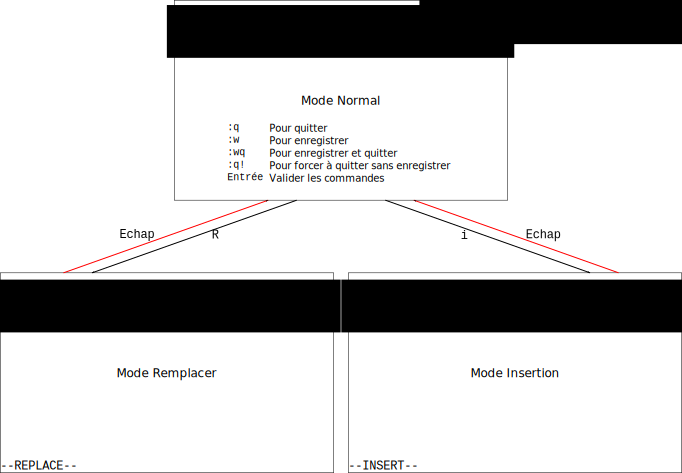
\includegraphics[width=0.7\linewidth]{vim_modes.pdf}
\caption{Modes principaux de \gras{vim} et comment passer de l'un à l'autre}
\end{figure}

\section{Se déplacer dans le document}
Dans le \gras[mode!Normal]{mode Normal}, les touches hjkl servent à se déplacer dans le document comme indiqué \reffig{fig:hjkl}. Les flèches directionnelles permettent de faire la même chose, l'avantage de \og hjkl\fg est que les touches sont plus proches et que c'est donc plus rapide à faire quand on a l'habitude (il parait).

\begin{figure}[htb]
\centering
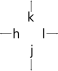
\includegraphics[width=0.25\linewidth]{vim_hjkl.pdf}
\caption{Les touches \texttt{hjkl} et comment se déplacer avec celles ci dans le mode \emph{Normal}}\label{fig:hjkl}
\end{figure}

\bigskip

\touche{Ctrl}+\touche{U} et \touche{Ctrl}+\touche{D} (respectivement Up et Down) permettent de se déplacer par page dans le document à raison d'une demi-page par appui (ça permet de continuer la lecture de manière plus fluide que si c'était une nouvelle page complète qui apparaissait, rendant plus difficile la lecture quand on n'a plus aucun point de repère).

\bigskip

Le raccourci \touche{Maj}+\touche{G} permet d'aller directement à la fin du document. Si vous faites\\
\touche{$n$}+\touche{Maj}+\touche{G} où $n$ est un nombre quelconque, le curseur est positionné à la ligne $n$. \touche{$1$}+\touche{Maj}+\touche{G} permet donc d'aller au début du document.


\section{Les différents modes d'édition}
\subsection{Modes \og persistants\fg}
Un mode \emph{persistant} est un mode que l'on active par appui sur une touche et dans lequel on reste jusqu'à ce qu'on appui sur la touche \touche{Échap}.

\bigskip

Le \gras[mode!Insertion]{mode Insertion} (\touche{i}) est le mode le plus courant, il permet d'écrire et d'effacer du texte comme le ferait un éditeur de texte normal.

Le \gras[mode!Append]{mode Append} (\touche{a}) fait exactement la même chose à part que le curseur d'édition est placé après le caractère courant sur lequel on était au moment de l'activation du mode.

\touche{o} permet de rentrer dans le mode Insertion en allant automatiquement sur une nouvelle ligne suivant la ligne courante (peu importe qu'on soit à la fin ou pas de la ligne, il ne découpe pas la ligne courante).

\bigskip

Le \gras[mode!Remplacement]{mode Remplacement} (\touche{R}) est un mode dans lequel le texte n'est pas inséré mais remplace le texte existant. C'est la même chose que le \gras[mode!Remplacer Caractère]{mode Remplacer Caractère} (à part que le \gras[mode!Remplacer Caractère]{mode Remplacer Caractère}, \touche{r}, ne permet de remplacer qu'un seul caractère).

\subsection{Modes \og un seul caractère\fg}
\begin{remarque}
Ces modes permettent d'agir sur un seul caratère, soit en le supprimant, le remplaçant ou autre.
\end{remarque}

Le \gras[mode!Remplacer Caractère]{mode Remplacer Caractère} (\touche{r}), permet de remplacer un caractère, celui en dessous du curseur.

Le \gras[mode!Supprimer Caractère]{mode Supprimer Caractère} (\touche{x}) supprime le caractère sous le curseur.


\section{Rechercher du texte}
Dans le \gras[mode!Normal]{mode Normal}, un appui sur \touche{/} permet de recherche le texte que l'on s'apprête à écrire. En résumé, pour rechercher \emph{texte}, il suffit d'écrire :
\begin{verbatim}
/texte
\end{verbatim}
Des appuis successifs sur \touche{n} (pour next) permettent d'aller aux occurences suivantes.

\section{Commandes dans le mode Normal}
Avant toute chose, la commande \touche{u} permet d'annuler une ou plusieurs commandes précédentes, effacement de texte ou autre.

\bigskip

Dans le \gras[mode!Normal]{mode Normal}, il existe quelque chose d'extrêmement puissant, c'est l'association de commande et d'objets. Ces \gras[commande-objet]{commande-objets} ont la forme suivante :
\begin{verbatim}
[nombre] commande objet
\end{verbatim}
où \verb|[nombre]| est facultatif et permet de répéter l'association \gras{commande-objet}.

\texttt{commande} est une commande de vim, il en existe surement plusieurs mais je ne connais que \texttt{d} pour l'instant, la commande d'effacement.

\texttt{objet} représente ce sur quoi va s'appliquer la commande, par exemple :
\begin{itemize}
\item\textbf{w} est un mot, le mot courant situé sous le curseur
\item\textbf{\$} est la fin de la ligne (C'est comme ça qu'elle est représentée dans les \gras{expression régulière}).
\item\textbf{\^} est le début de la ligne (C'est comme ça qu'elle est représentée dans les \gras{expression régulière}).
\end{itemize}

Ainsi \texttt{dw}, \texttt{d\$} et \texttt{d\^} vont effacer respectivement le mot courant, jusqu'à la fin de la ligne, jusqu'au début de la ligne.

La commande \texttt{dd} quant à elle permet d'effacer la ligne courante.

\begin{remarque}
La commande \texttt{p} permet de coller ce qui vient d'être effacé.
\end{remarque}


\bigskip

L'autre type de commande, ce sont celles commençant par un double point \og :\fg. Par exemple les commandes \texttt{:q}, \texttt{:q!} et \texttt{:wq} permettent respectivement de quitter, forcer à quitter (quand il y a eu des modifications que l'on ne souhaite pas sauvegarder, et sauvegarder puis quitter.
\begin{itemize}
\item \texttt{:w} pour sauvegarder
\item \texttt{:q} pour quitter
\item \texttt{:q!} pour forcer à quitter (quand il y a eu des modifications que l'on ne souhaite pas sauvegarder)
\item \texttt{:wq} pour sauvegarder puis quitter
\end{itemize}

\begin{attention}
Ces commandes ne peuvent être entrées QUE dans le \gras[mode!Normal]{mode Normal}, c'est à dire celui où écrire du texte l'affiche en bas à gauche. Ce \gras[mode!Normal]{mode Normal} pourrait aussi s'appeler le \gras[mode!Commande]{mode Commande}
\end{attention}

\clearpage
\printindex
\end{document}